\chapter{Unorganized Text}

\todo{Remove this chapter}

This chapter serves as a collection of text fragments that have not yet been assigned to a particular chapter.

\section{Monitoring}

The three pillars of observability \cite{9837035}
\begin{itemize}
    \item Metrics
    \item Logs
    \item Traces
\end{itemize}

Because of the scope of this work, only the pillar of Metrics is considered.

\begin{quote}
\textit{``Metrics are numerical representations of data that Ops teams use to determine the overall behavior of a system, service, or network component over time.'', \cite{9837035}}
\end{quote}

The four golden signals \cite{Beyer2016-xi}
\begin{itemize}
    \item Latency: time to service a request
    \item Traffic: requests per second
    \item Errors: rate of failed requests
    \item Saturation: how saturated are constrained resources like memory or I/O
\end{itemize}

White-box vs. Black-box Monitoring \cite{Beyer2016-xi}
\begin{itemize}
    \item White-box: Monitoring based on internal system metrics.
    \item Black-box: Monitoring based on externally visible behavior.
\end{itemize}

Internal vs. External resources in a monitoring context:
Internal resources describe resources that allow direct access to their internals.
An example of an internal resource is a self-hosted microservice.
External resources describe resources that do not allow direct access to their internals.
An example of an external resource is a Software-as-a-Service (SaaS) product which is used in a context that should be monitored.

External resources can, because of their nature, only be monitored using the Black-box approach.
Internal resources however can be monitored with both the White-box and Black-box approach.

Motivations for monitoring cloud applications \cite{6483656}
\begin{itemize}
    \item Capacity and Resource Planning
    \item Capacity and Resource Management
    \item Data Center Management
    \item SLA Management
    \item Billing
    \item Troubleshooting
    \item Performance Management
    \item Security Management
\end{itemize}

\todo{Capacity and Resource Planning}

\todo{Capacity and Resource Management}

Data Center Management is mainly concerned with the efficient usage of resources.
One key measurement of the efficiency of a data center is its energy efficiency.

SLA Management refers to the monitoring of parameters, which are defined in Service Level Agreements (SLA).
These parameters must be within set bounds for an SLA to be considered fulfilled.

Billing refers to the monitoring of parameters that influence the cost of running an application.
When an application is hosted on a cloud provider's Infrastructure-as-a-Service (IaaS) system,
one of those parameters might be the number of compute instances that an application uses.

While Troubleshooting usually refers to the tracing of requests and failures to provide a dataset for analyzing and fixing issues in an application,
Monitoring can also be used to aid in troubleshooting by recording the number of failed requests and their context.

\todo{Performance Management}

\todo{Security Management}

\section{Monitoring BestRental}

\subsection{Monitoring Targets}

Figure \ref{fig:sps_architecture_bestrental} shows the System Plus Software Architecture of the Demonstrator BestRental.

\begin{figure}
	\centering
	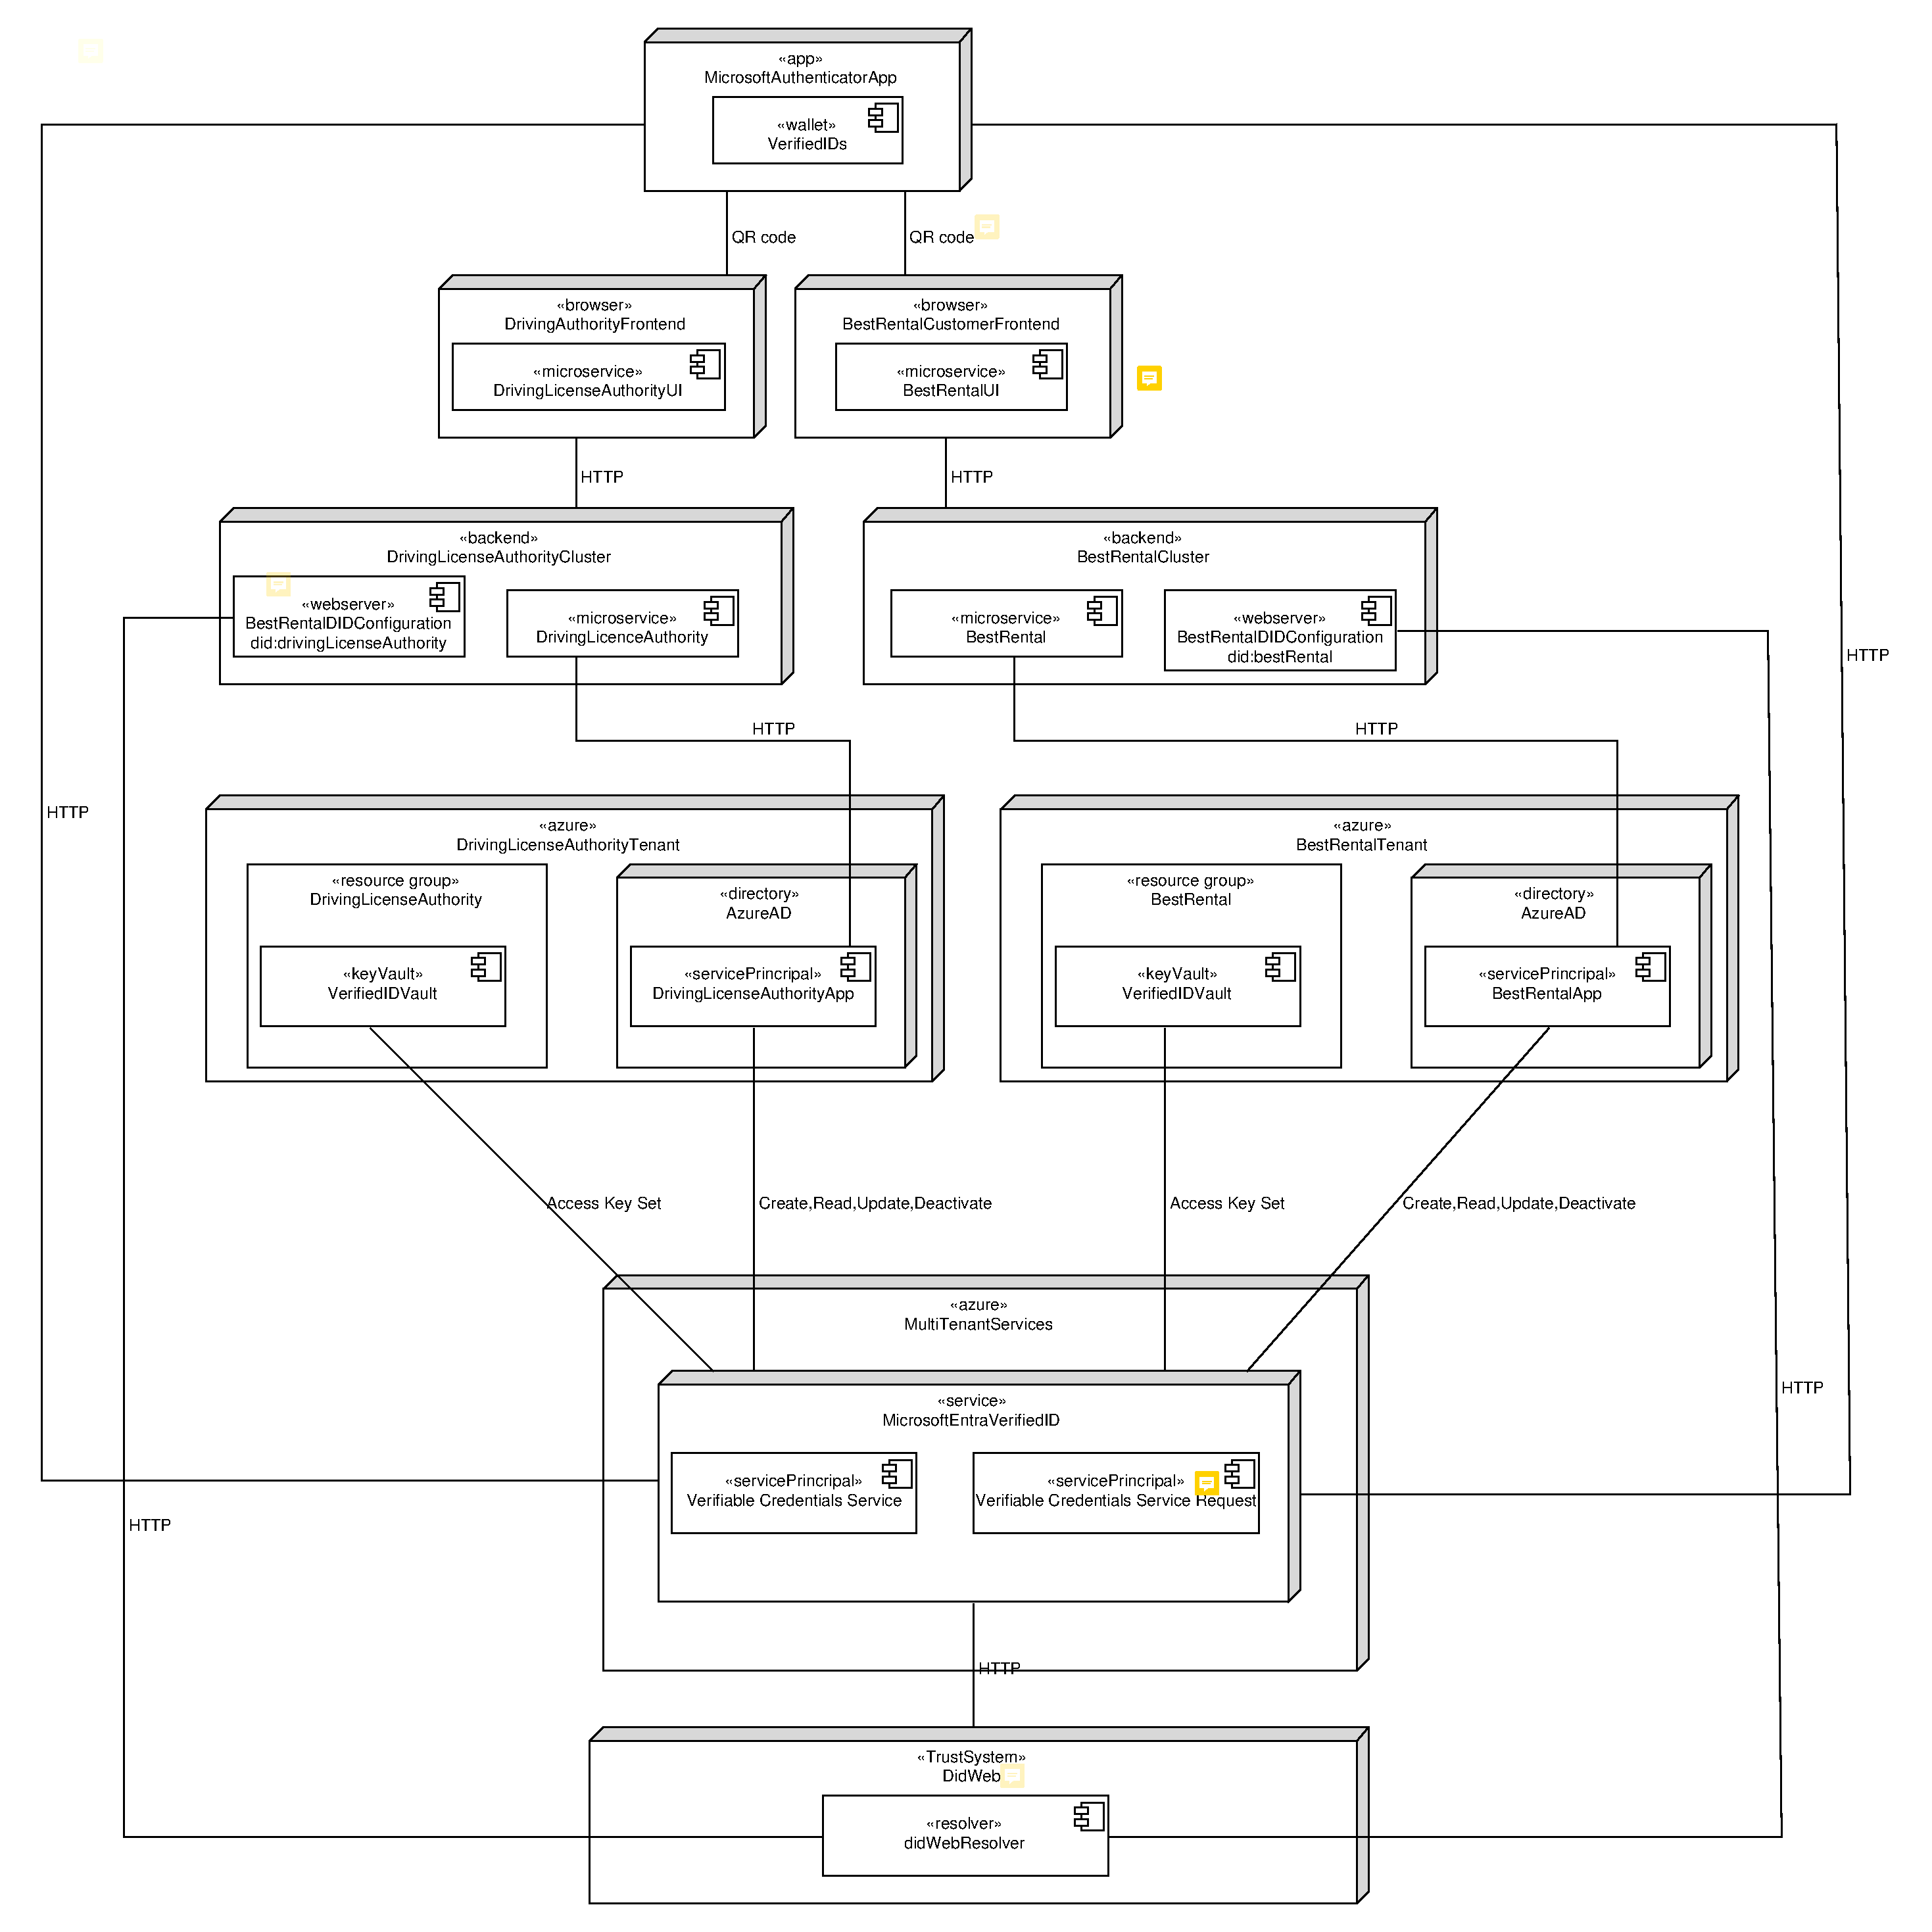
\includegraphics[width=\textwidth]{pdfs/sps_achitecture_bestrental.pdf}
	\caption{System Plus Software Architecture BestRental}
	\label{fig:sps_architecture_bestrental}
\end{figure}

The Demonstrator for BestRental includes multiple types of resources.
These can be grouped into internal and external resources.
\begin{enumerate}
    \item Microsoft Application: External
    \item Service: Internal
    \item Cluster: Internal
    \item Azure Tenant: External
    \item Azure Resource Group: External
    \item Azure Directory: External
    \item Service (Principal): External
    \item Trust System: External
    \item Trust Resolver: External
\end{enumerate}

For the collection of metrics from external Microsoft Azure resources, the service Azure Monitor can be used.
This service allows the export and import through a REST API.

\begin{table}[]
\begin{tabular}{ll}
   & Requirement       \\
R1 & High Availability \\
R2 & Scalability       \\
R3 & Extensibility    
\end{tabular}
\caption{Requirements for a Monitoring Solution}
\label{tab:requirements}
\end{table}

\begin{table}[]
\begin{tabular}{ll}
     & Objective                                   \\
QoS1 & Application uptime                          \\
QoS2 & Maximum latency                             \\
\end{tabular}
\caption{Quality of Service Objectives}
\label{tab:qos_objectives}
\end{table}

\begin{table}[]
\begin{tabular}{llll}
    & Metric                                             & Motivation                       & Internal/External resources/Application \\
M01 & Active Sessions                                    & Performance Management           & Application                             \\
M02 & Login attempts                                     & Security Management              & Application                             \\
M03 & Average failed login attempts per session          & Security Management              & Application                             \\
M04 & Maximum failed login attempts per session          & Security Management              & Application                             \\
M05 & Total incoming requests per hour                   & Performance Management           & Application                             \\
M06 & Average incoming requests per session per hour     & Performance Management           & Application                             \\
M07 & Average incoming requests per service per hour     & Performance Management           & Internal                                \\
M08 & Average outgoing requests per service per hour     & Performance Management           & Internal                                \\
M09 & Total failed requests                              & SLA Management                   & Application                             \\
M10 & Total failed requests per service                  & Troubleshooting                  & Internal/External                       \\
M11 & Average failed requests per session                & SLA Management                   & Application                             \\
M12 & Average latency for incoming requests              & SLA Management                   & Application                             \\
M13 & Average latency between services                   & Performance Management           & Internal                                \\
M14 & Maximum resource usage of service                  & Capacity and Resource Management & Internal                                \\
M15 & Average resource usage of service in the last hour & Capacity and Resource Management & Internal                                \\
M16 & Total accumulated cost                             & Billing                          & Application                             \\
M17 & Accumulated cost per service                       & Billing                          & Internal/External                       \\
M18 & Total application downtime                         & SLA Management                   & Application                             \\
M19 & Downtime per service                               & SLA Management                   & Internal/External                      
\end{tabular}
\caption{Monitoring Metrics}
\label{tab:monitoring_metrics}
\end{table}